\section{Supernova explosion}

\begin{frame}{3D RHD simulations (Longo et al. 2025)}
	\begin{columns}

		{\footnotesize
		\begin{column}{0.5\textwidth}
		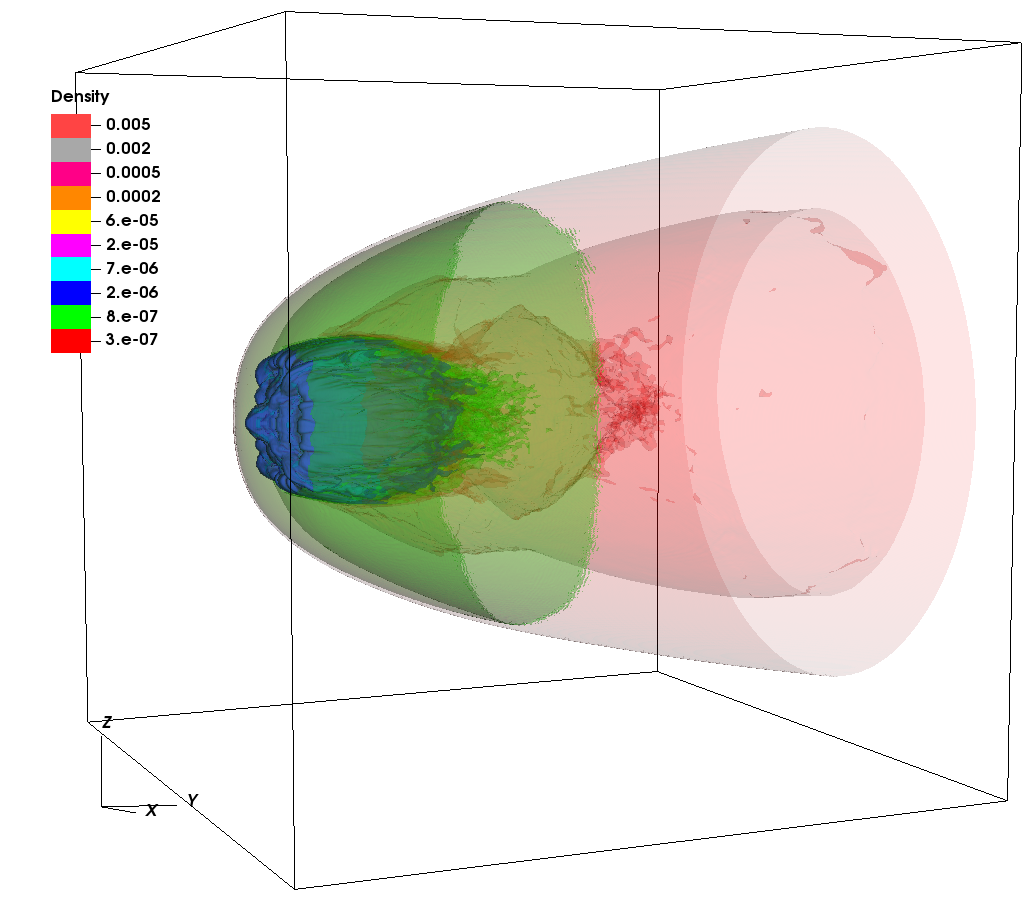
\includegraphics[width=\textwidth]{images/3d_shot_rho.png}
				\vspace{-.5cm}
		 \begin{itemize}
		  \item We start $\approx 10^{3}\,{\rm yr}$ post explosion,
		 				located far from the jet walls
		  \item $R_{\rm j} >> R_{\rm SN}\quad \Rightarrow R_{\rm SN}\approx 10^{-2} R_{\rm j}$ \\
		  \item  Uniform ejecta $\rho_{\rm SN},p_{\rm SN}>>\rho_{\rm j},p_{\rm j}$
		  \item Jet and ejecta: ionized gas of protons and electrons
		 \end{itemize}

		\end{column}}
		\begin{column}{0.7\textwidth}
			{\scriptsize
		 \begin{columns}\begin{column}{.5\textwidth}
		  \begin{alertblock}{Jet properties}
			\begin{itemize}
		      \item $R_{\rm j} = 100\,{\rm pc}$
			  \item $L_{\rm j} = 10^{44}\,{\rm erg}\,{\rm s}^{-1}$
			  \item $\Gamma_{\rm j}=2$
			  \item $h_{\rm j} = 1.1c^{2}$
			  \item $\rho_{\rm j} = 6\cdot10^{-30}\,{\rm g}/{\rm cm}^{3}$
			  \item $T_{\rm j} = 2\times 10^{11} K$
			\end{itemize}
		   \end{alertblock}
		  \end{column}
		  \hspace{-2cm}
		  \begin{column}{.5\textwidth}
		   \begin{exampleblock}{SN properties}
		     \begin{itemize}
					\item $M_{\rm SN}=2\,M_\odot$
					\item $E_{\rm SN}=10^{51}\,{\rm erg}$
					\item $R_{\rm SN}=1.1\,{\rm pc}$
					\item $\rho_{\rm SN}= 2.4\cdot10^{-23}\,{\rm g}/{\rm cm}^{3}$
					\item $T_{\rm SN} = 10^{9}\,K$
					\item $v_{\rm orb} = 200\,{\rm km}\,{\rm s}^{-1}$
				\end{itemize}
			\end{exampleblock}
		 \end{column}
		\end{columns}}
		\vspace{1cm}
		{\scriptsize
		\begin{block}{Code: \texttt{Ratpenat} (Perucho 2010)}
			OpenMPI+OpenMP HRSC 3D RHD code, Marquina 1998 fluxes, PPM recon, Synge equation
			\\
				Conservative form equations $\frac{\partial U}{\partial t}+\frac{F^{i}}{\partial x^{i}}=0$\\
				Where $U=(D,S^{j},\tau)^{T}$ and $F = (Dv^{i}, S^{j}v^{i}+p\delta^{ij}, S^{i}-Dv^{i}) $
		\end{block}
			}
		\end{column}
	\end{columns}
\end{frame}
\begin{frame}{2D cuts through the 3D physical domain}
\begin{columns}
	\begin{column}{.9\textwidth}
	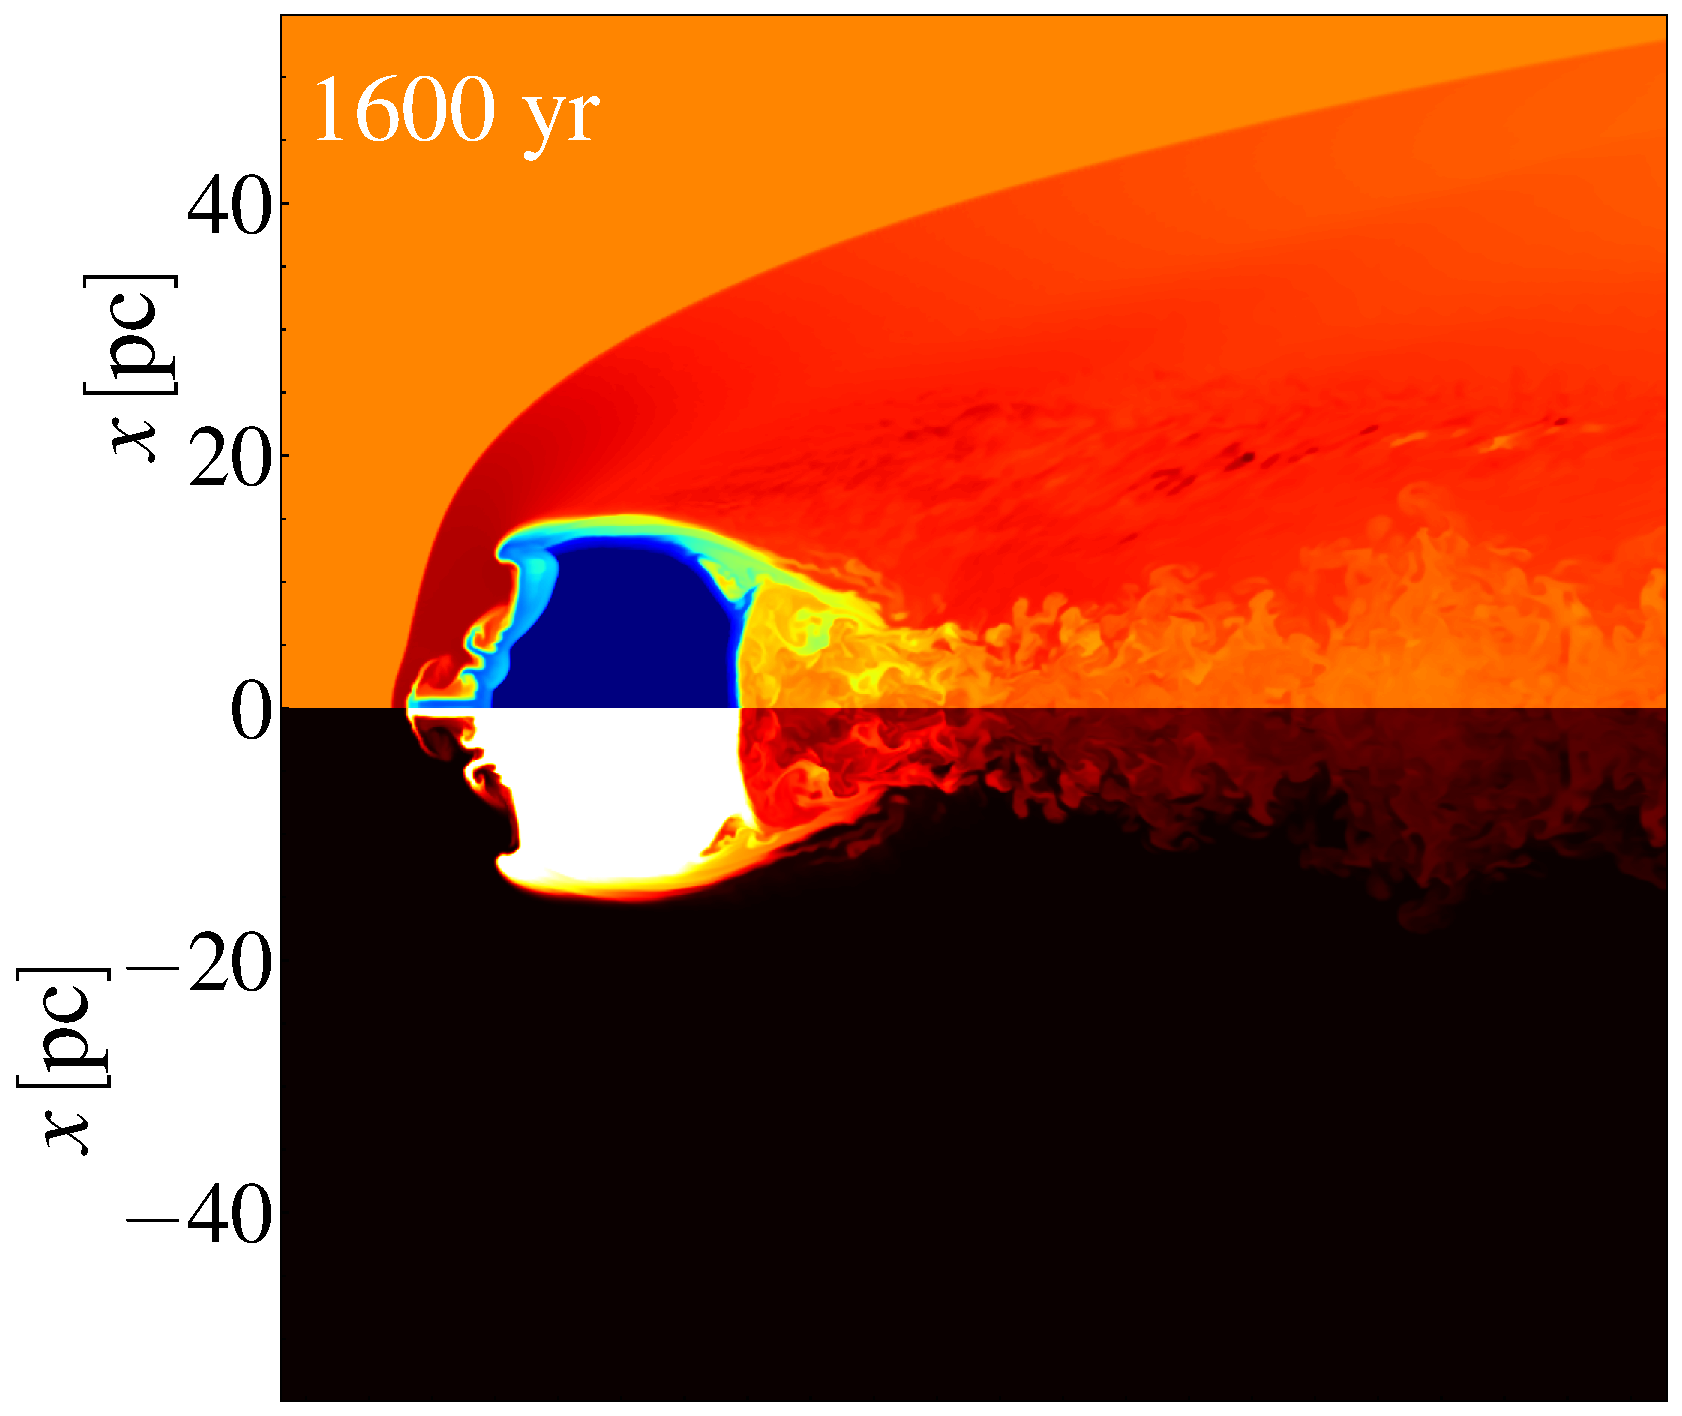
\includegraphics[width=0.3612\linewidth]{images/2d_tem_trac_450.pdf}
	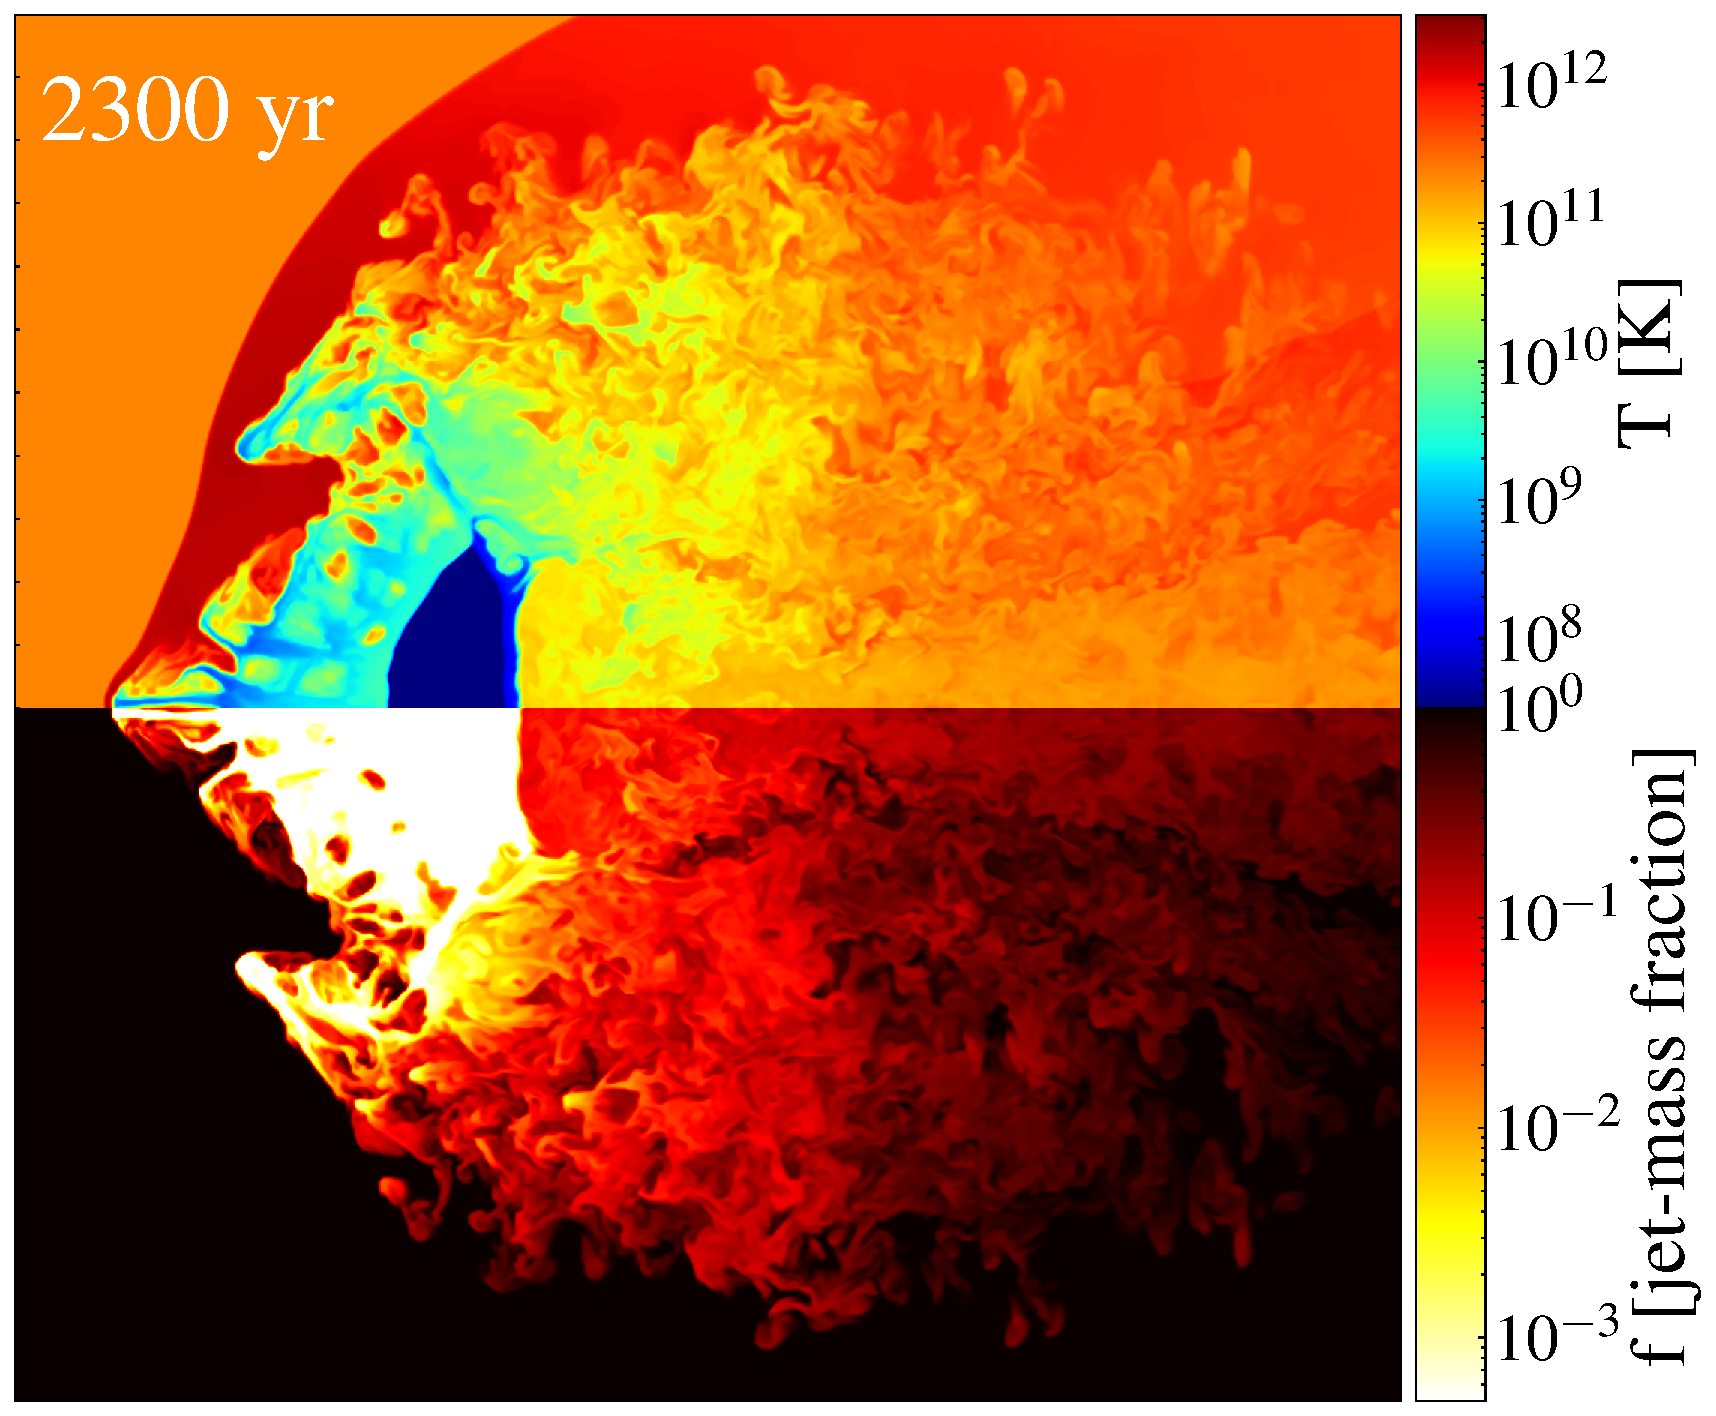
\includegraphics[width=0.3675\linewidth]{images/2d_tem_trac_650.pdf} \\
	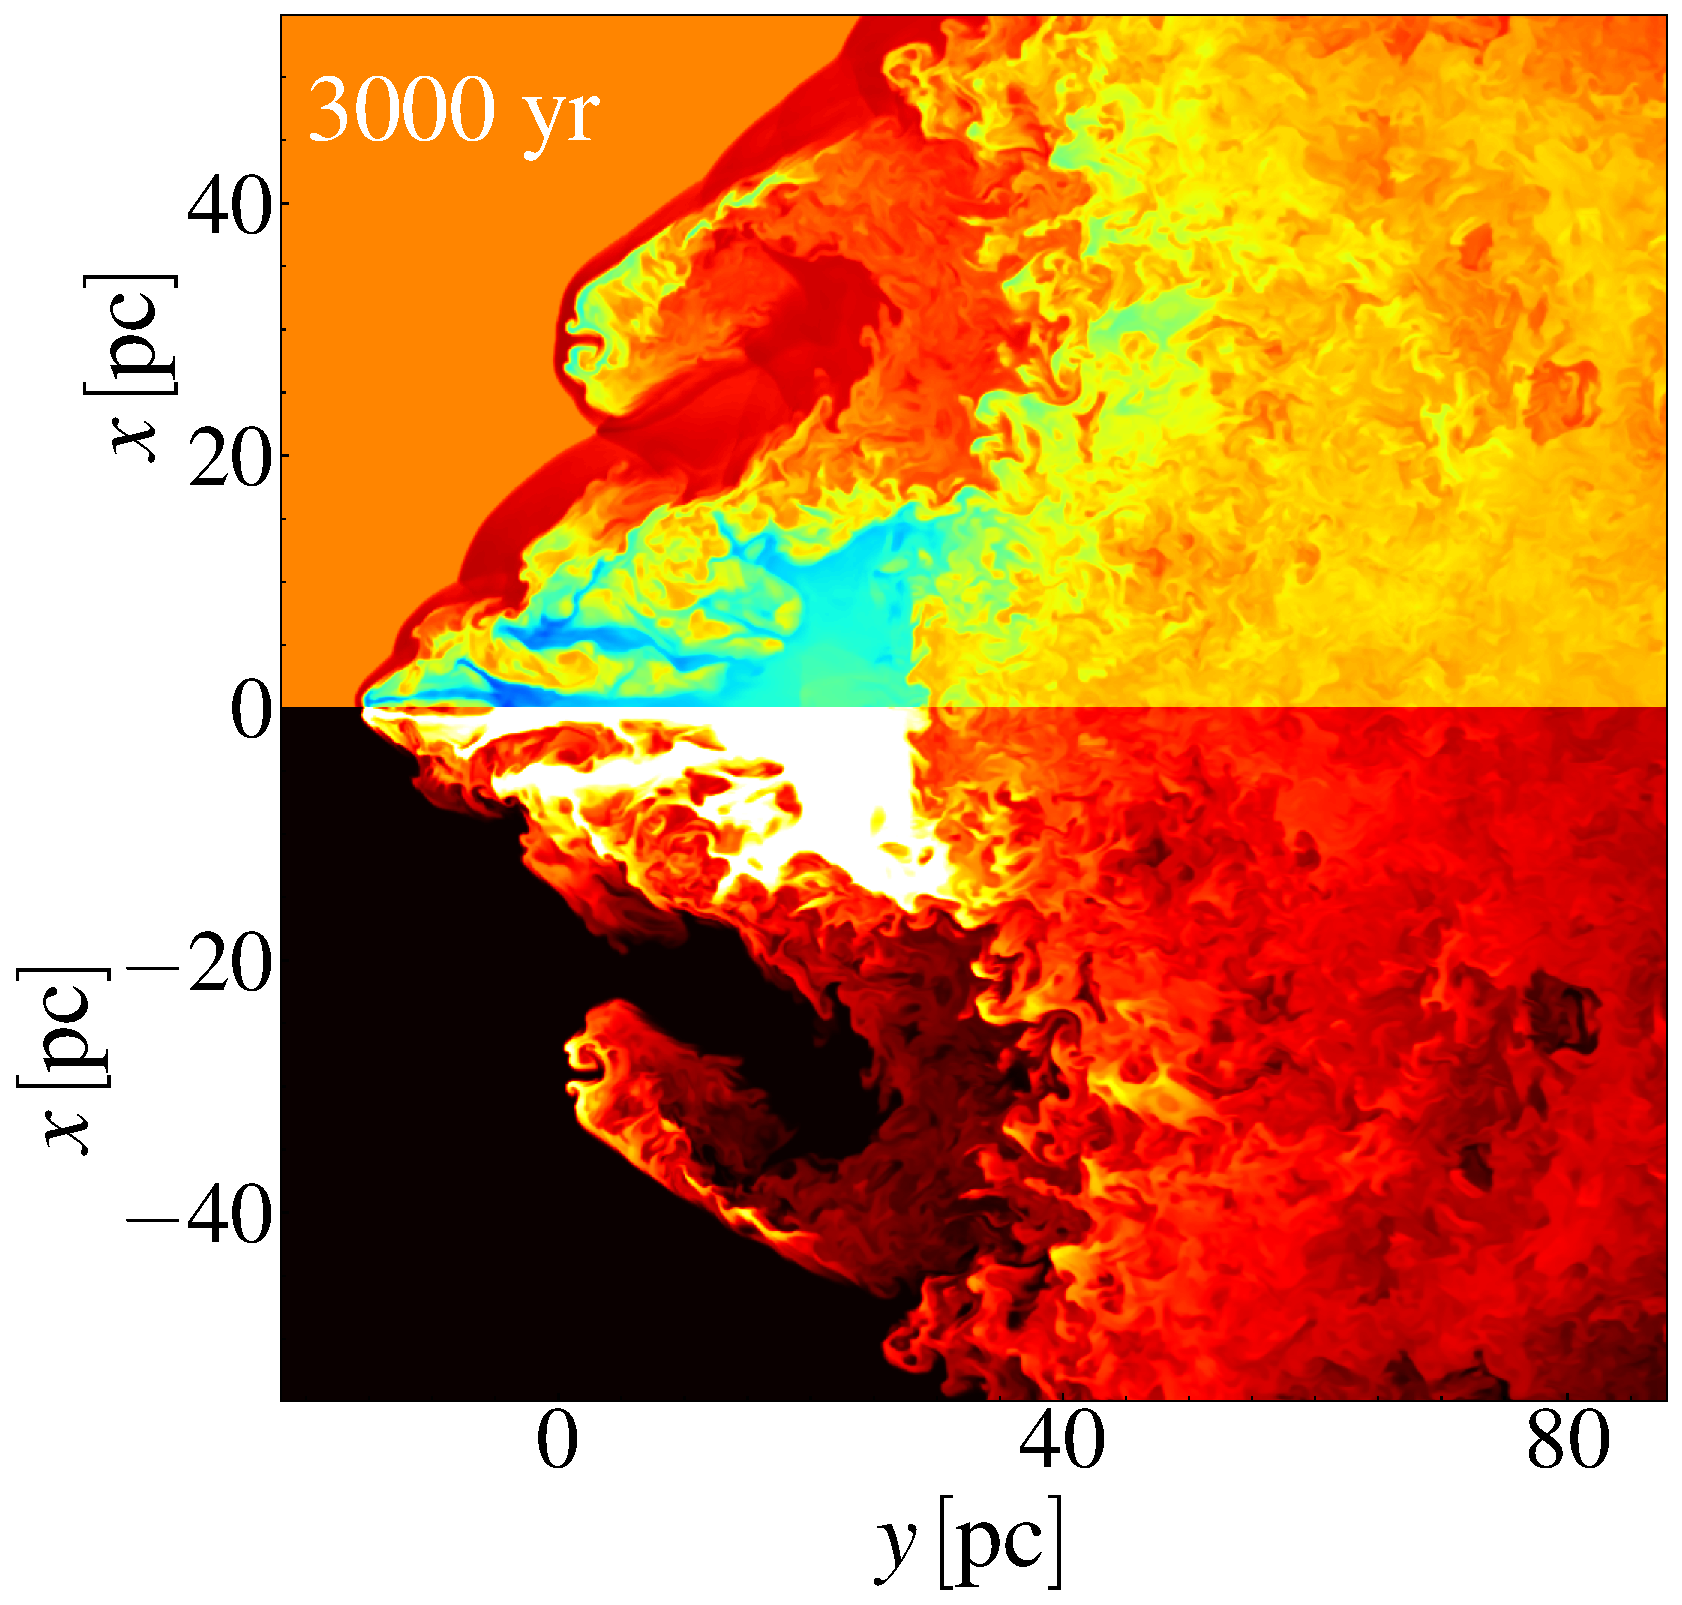
\includegraphics[width=0.36015\linewidth]{images/2d_tem_trac_850.pdf}
	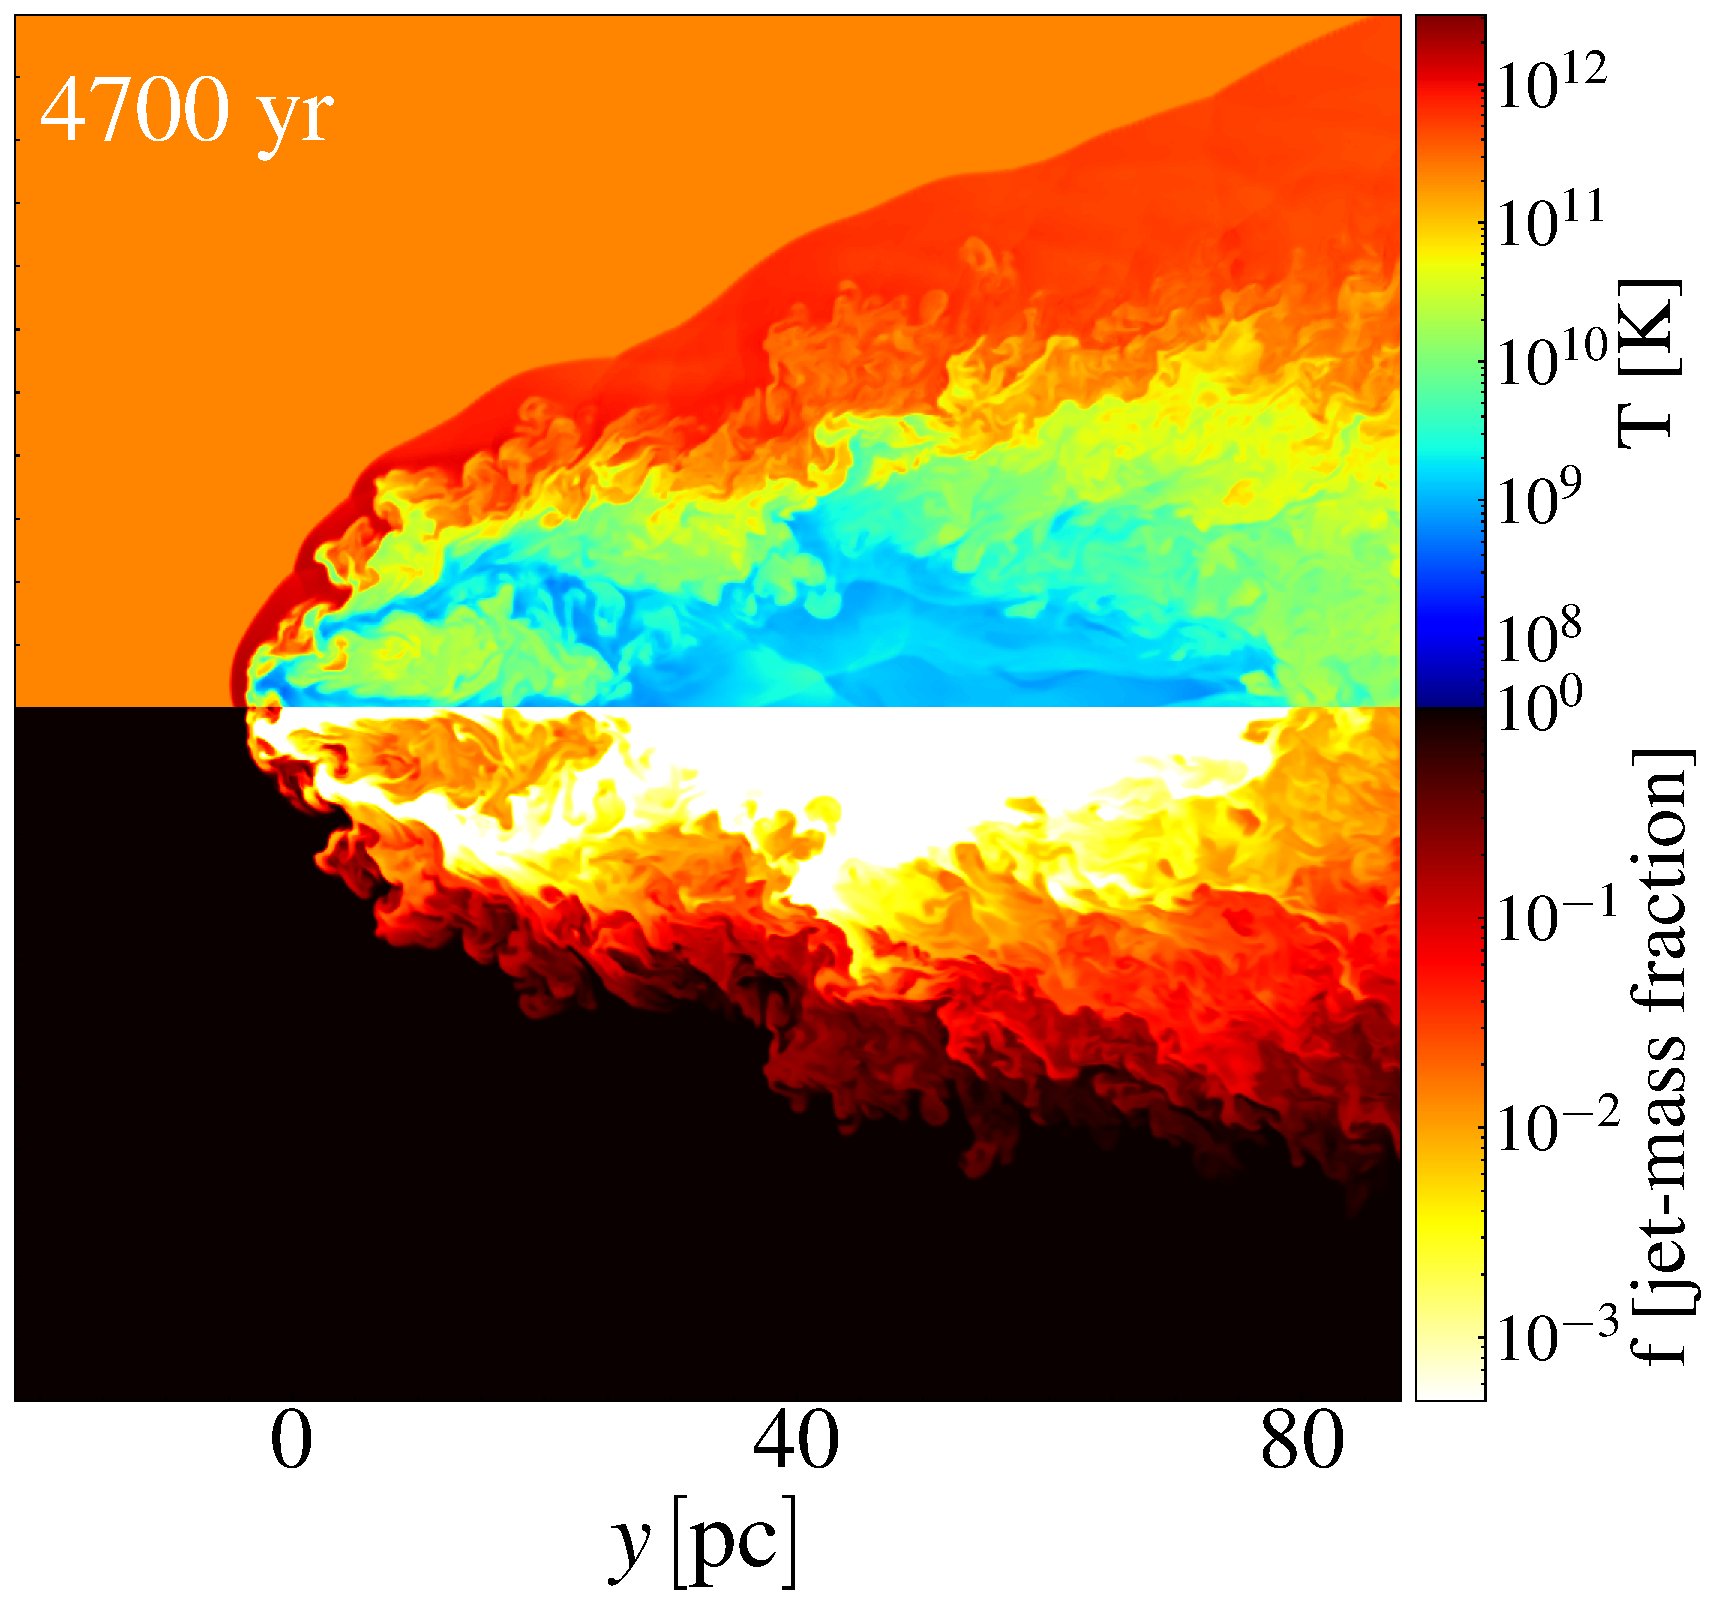
\includegraphics[width=0.36855\linewidth]{images/2d_tem_trac_1300.pdf}
	\end{column}
	\hspace{-3cm}
	\begin{column}{.4\textwidth}
			\begin{block}{Dynamical evolution}
	{\footnotesize
	\begin{itemize}
		\item Free expansion phase
		\item Shock wave and disruption
		\item Important mixing
		\item Ejecta swept away
	\end{itemize}
	}
	\end{block}
	\end{column}
	\end{columns}
\end{frame}
\section{Non-thermal emissions}

\begin{frame}{Non-thermal emission:\\
	Simplified approach to compute the radiative output}
	\begin{columns}
		{\scriptsize
		\begin{column}{.5\textwidth}
			\begin{block}{Power emitted}
				\begin{itemize}
					\item Non-thermal energy $E_{\rm NT} = \eta U_{\rm cell}$ where $\eta<1$
					\item Broken power-law for the e$^{-}$ distribution with a break 
							energy given by the adiabatic time  \\
					\item Inverse Compton scattering + Synchrotron
				\end{itemize}
			\end{block}
			\begin{block}{Inverse Compton scattering}
			    \begin{itemize}
				    \item Target photons:\\
						$\rightarrow$ Anisotropic CMB + IR galactic background
					\item Approximate formula for the Thompson+Klein-Nishina regime
						(Khangulyan 2014, Bosch-Ramon 2018)
				\end{itemize}
			\end{block}
		\end{column}
		\begin{column}{.5\textwidth}
			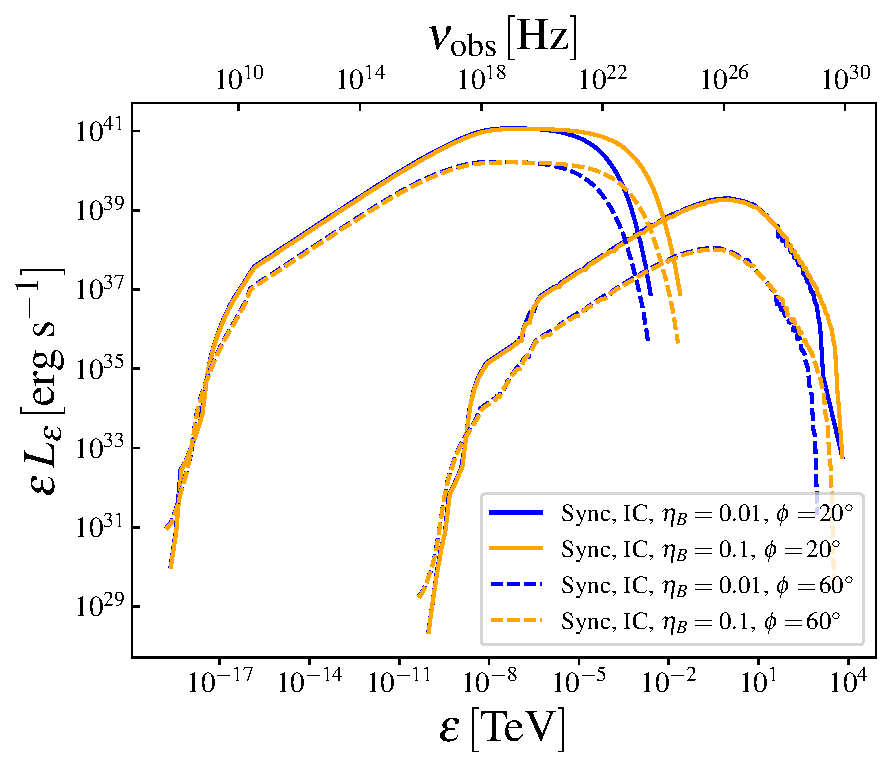
\includegraphics[width=\linewidth]{images/eled_hr.pdf}
			\begin{exampleblock}{Emitted luminosity}
				\begin{itemize}
					\item With the given e$^{-}$ distribution, we reach the PeV in IC
					\item The Synchrotron emission reaches $10^{41}\,{\rm erg}\,{\rm s}^{-1}$
							and the IC $10^{39}\,{\rm erg}\,{\rm s}^{-1}$
				\end{itemize}
			\end{exampleblock}
			\centering
		\end{column}
		}
	\end{columns}
\end{frame}
\begin{frame}{Flux on the line of sight for a source at $z=0.007$ and $\phi=20$°}
	\begin{columns}
		\begin{column}{0.1\textwidth}
				{\small {\bf IC} \\$10^{27}\,{\rm Hz}$  }
		\end{column}
		\begin{column}{\textwidth}
	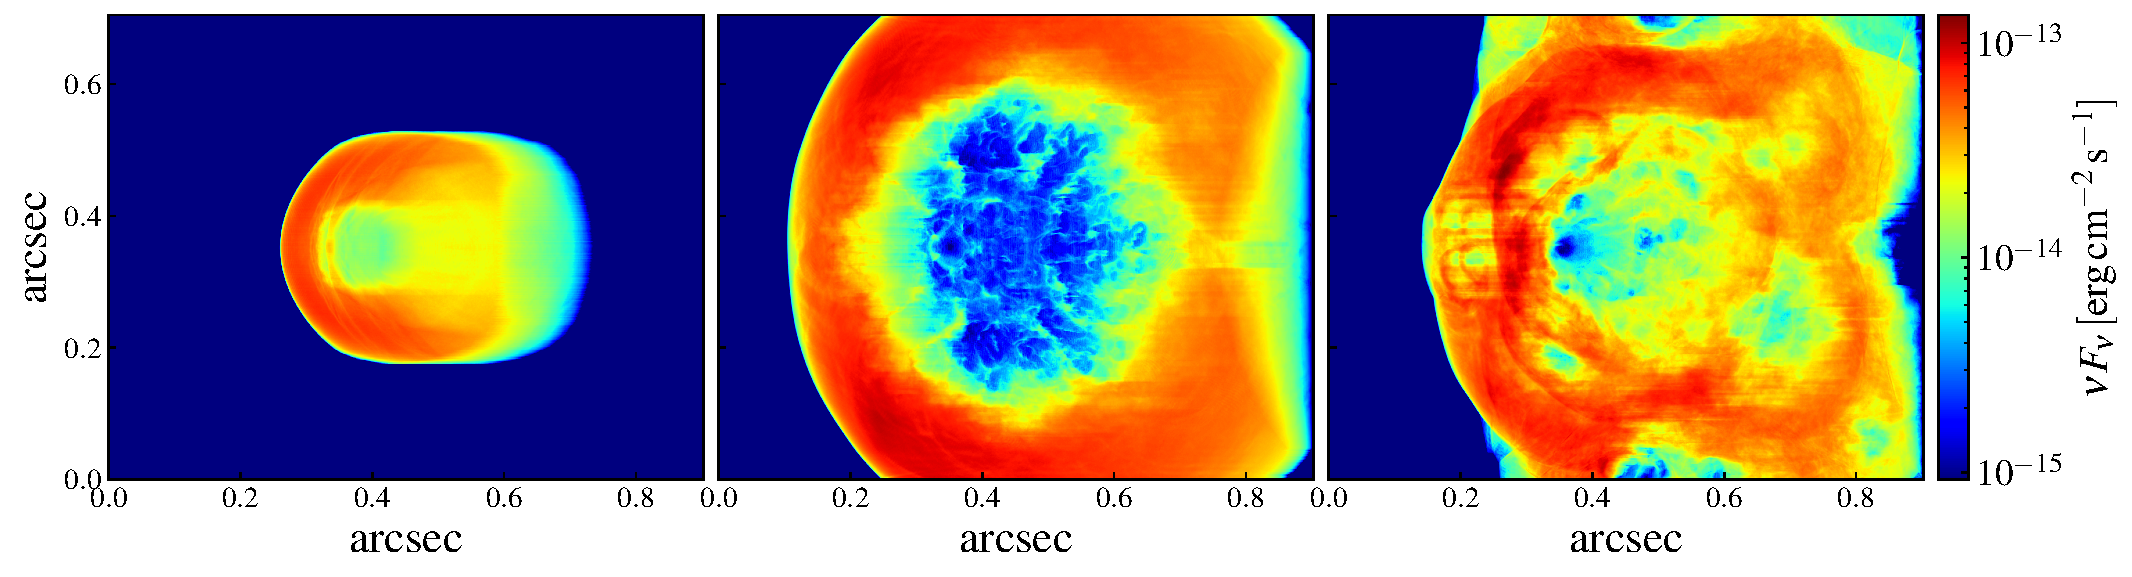
\includegraphics[width=\linewidth]{images/2dmaps/2Dmap_flux_freq_27_dist_31_phi_20_ic.pdf}
		\end{column}
	\end{columns}
	\begin{columns}
		\begin{column}{0.1\textwidth}
				{\small{\bf Sync} \\ $10^{10}\,{\rm Hz}$}
		\end{column}
		\begin{column}{\textwidth}

	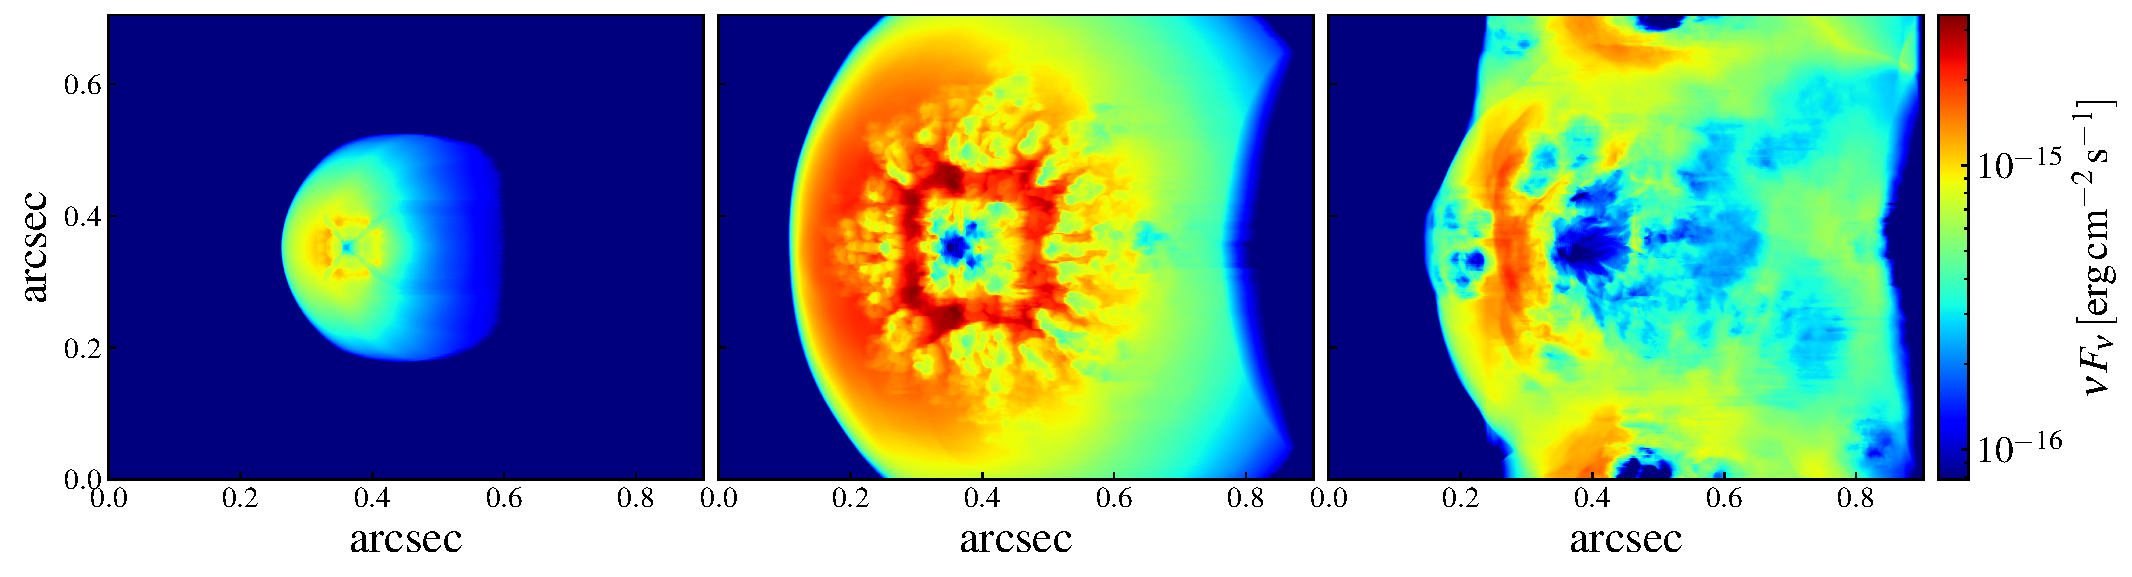
\includegraphics[width=\linewidth]{images/2dmaps/2Dmap_flux_freq_10_dist_31_phi_20_sync.pdf}
		\end{column}
	\end{columns}
	\vspace{8pt}
		\hspace{70pt} $1\,{\rm kyr}$ \hspace{60pt} $2.3\,{\rm kyr}$ \hspace{60pt} $3.8\,{\rm kyr}$
\end{frame}

\begin{frame}{Flux on the line of sight for a source at $z=0.007$ and $\phi=60$°}
	\begin{columns}
		\begin{column}{0.1\textwidth}
				{\small {\bf IC} \\$10^{24}\,{\rm Hz}$  }
		\end{column}
		\begin{column}{\textwidth}
	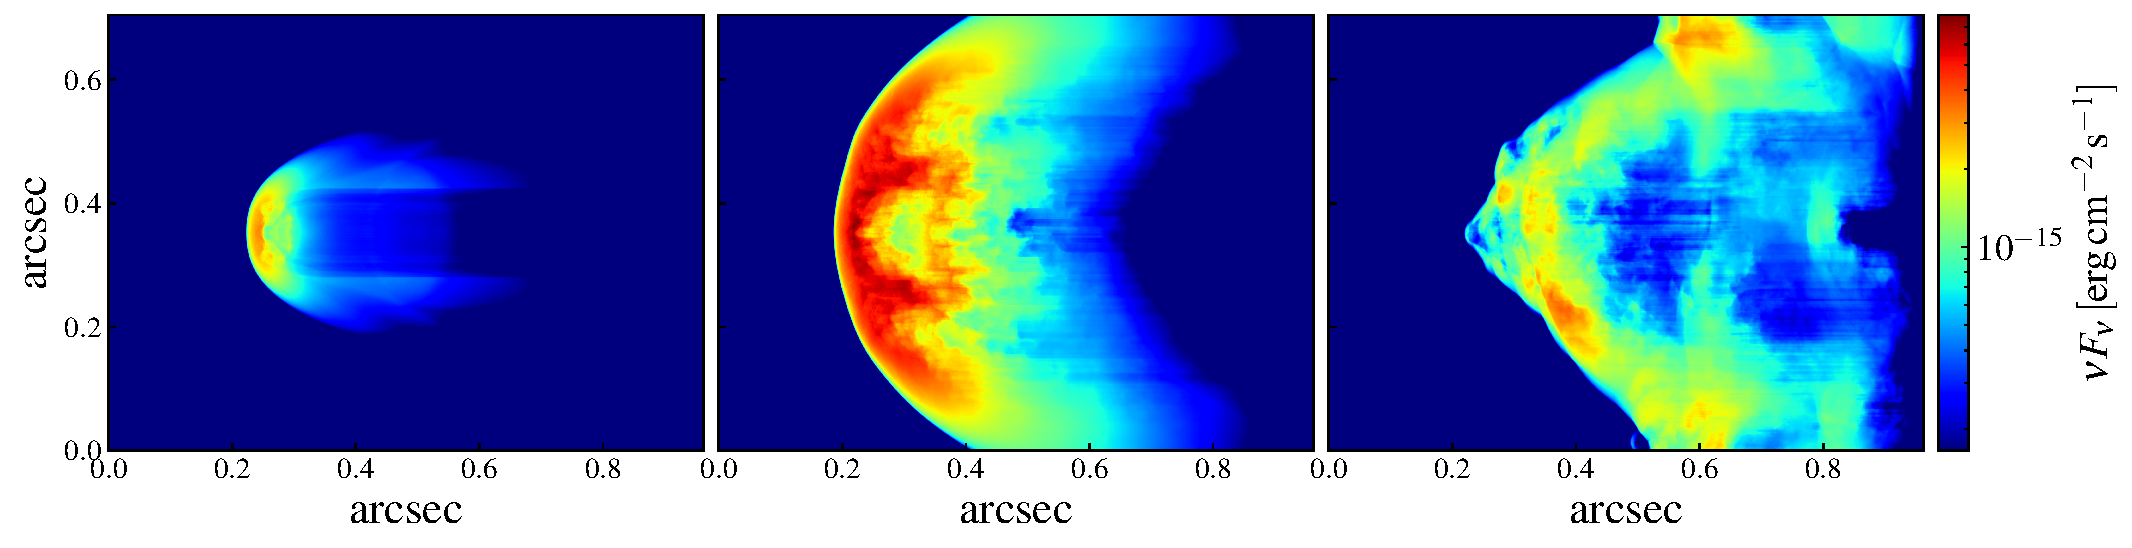
\includegraphics[width=\linewidth]{images/2dmaps/2Dmap_flux_freq_24_dist_31_phi_60_ic.pdf}
		\end{column}
	\end{columns}
	\begin{columns}
		\begin{column}{0.1\textwidth}
				{\small{\bf Sync} \\ $10^{18}\,{\rm Hz}$}
		\end{column}
		\begin{column}{\textwidth}

	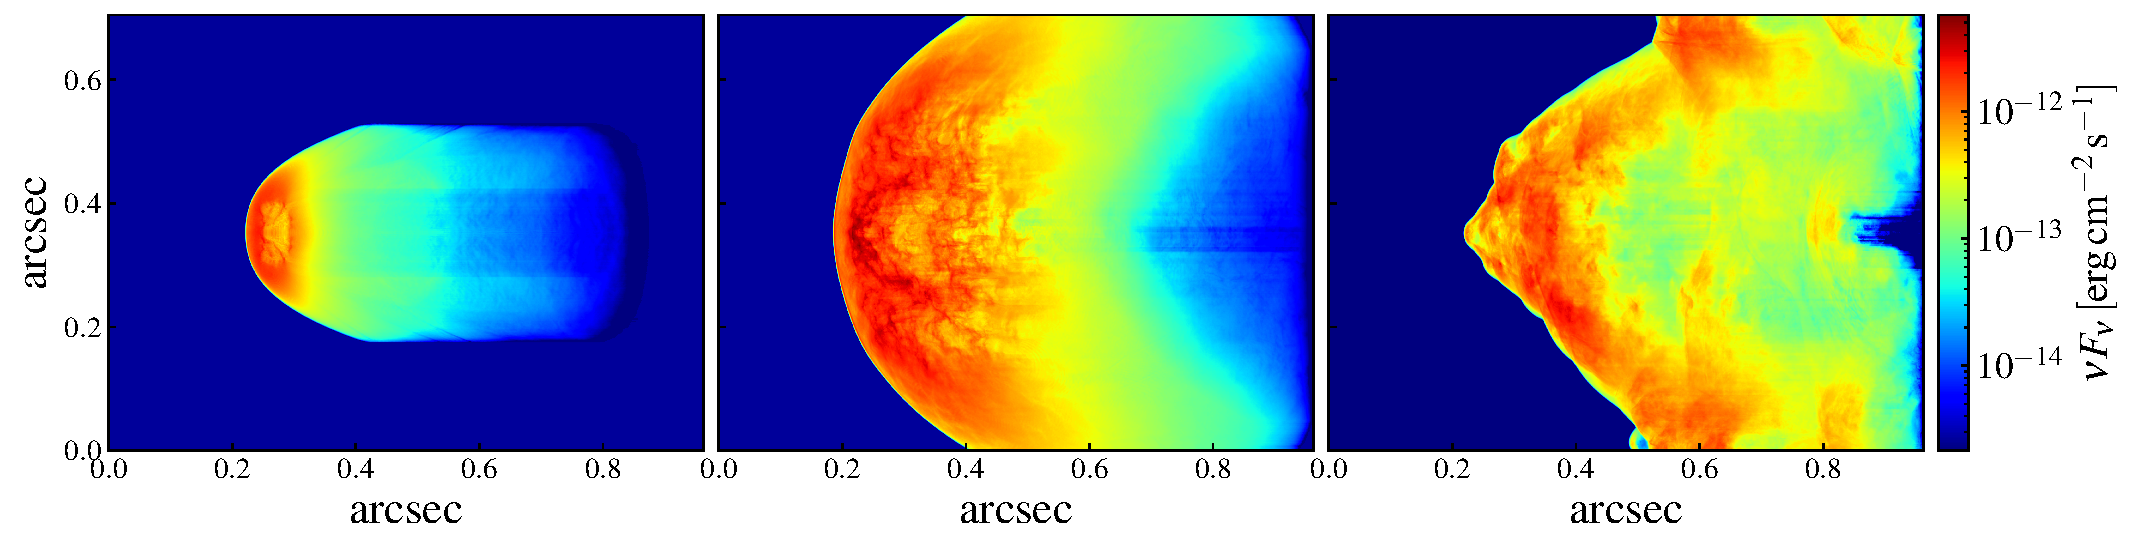
\includegraphics[width=\linewidth]{images/2dmaps/2Dmap_flux_freq_18_dist_31_phi_60_sync.pdf}
		\end{column}
	\end{columns}
	\vspace{8pt}
		\hspace{70pt} $1\,{\rm kyr}$ \hspace{60pt} $2.3\,{\rm kyr}$ \hspace{60pt} $3.8\,{\rm kyr}$
\end{frame}

\begin{frame}{SEDs with $\phi=20,60^{\circ}$}
	\begin{columns}
		\begin{column}{.6\textwidth}
			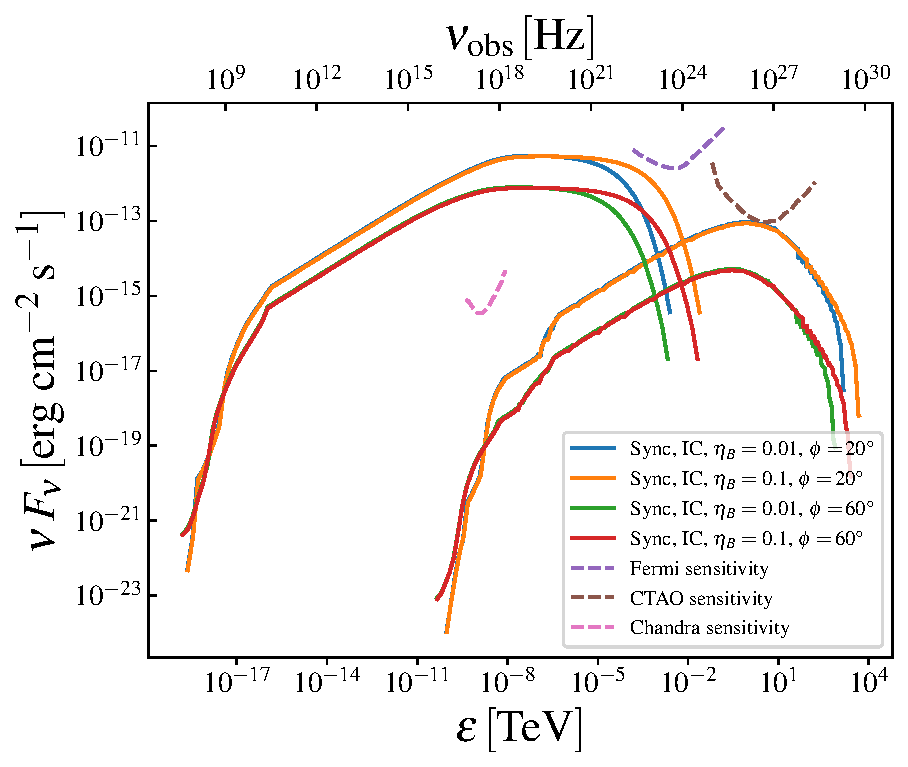
\includegraphics[width=\textwidth]{images/sed_hr.pdf}
		\end{column}
		\begin{column}{.4\textwidth}
			{\scriptsize
			\begin{itemize}
				\item Ratio $\eta_{\rm B}=p_{\rm B}/p_{\rm g}=10^{-2}$
				\item Source at $z=0.003\;(13{\rm Mpc})$ (type CenA)
				\item Fluxes for Synchrotron and IC emission
				\item Possible detecion of Sync by Chandra and IC by CTAO
			\end{itemize}
			}
		\end{column}
	\end{columns}
\end{frame}

\begin{frame}{Light curve with $\phi=20,60^{\circ}$ and $z=0.007\;(31{\rm Mpc})$}
	\begin{columns}
		\begin{column}{.5\textwidth}
		\centering
		{\scriptsize Xrays $(10^{18}\,{\rm GHz})$}
			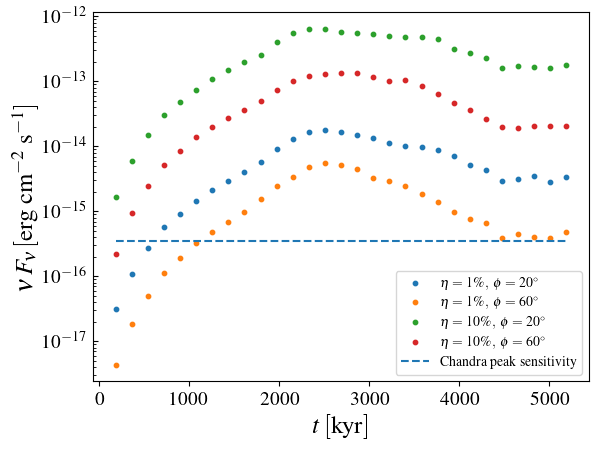
\includegraphics[width=.95\textwidth]{images/Chandra_Sync.png}
		\end{column}
		\begin{column}{.5\textwidth}
				\centering
          {\scriptsize $\gamma$-rays $(10^{27}\,{\rm GHz})$}
   	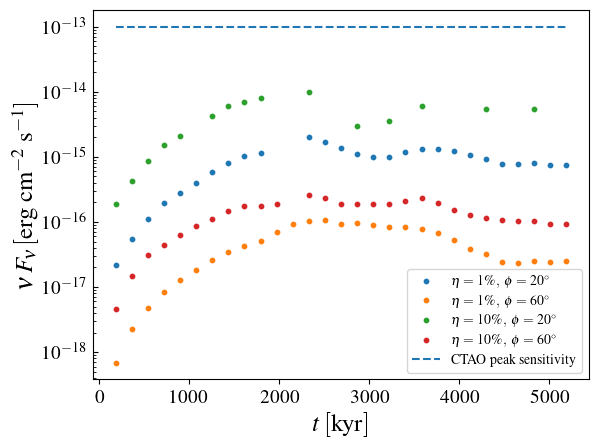
\includegraphics[width=.95\textwidth]{images/CTAO_IC.png}
		\end{column}
	\end{columns}
		{\scriptsize
			\begin{itemize}
				\item Internal to non-thermal energy ratio $\eta=0.1,0.01$
				\item IC close to be detectable in $\gamma$-rays
				\item Chandra is sensible enough to observe the Synchrotron emissions for the whole duration of the interaction
			\end{itemize}
		}
\end{frame}

